\documentclass[a4paper,twoside]{article}

\usepackage{epsfig}
\usepackage{subfigure}
\usepackage{calc}
\usepackage{amssymb}
\usepackage{amstext}
\usepackage{amsmath}
\usepackage{amsthm}
\usepackage{multicol}
\usepackage{pslatex}
\usepackage{apalike}

\usepackage{booktabs}
\usepackage{csquotes}

\usepackage{graphicx}
\graphicspath{{rsc/}}
\DeclareGraphicsExtensions{.pdf,.png,.eps}

\usepackage[utf8]{inputenc}

%\usepackage{algorithm}
%\usepackage[noend]{algpseudocode}

\usepackage{algorithm2e}

\usepackage{SCITEPRESS}     % Please add other packages that you may need BEFORE the SCITEPRESS.sty package.

\subfigtopskip=0pt
\subfigcapskip=0pt
\subfigbottomskip=0pt

\begin{document}

\title{Efficient Evidence Accumulation Clustering for large datasets}

\author{\authorname{Diogo Silva\sup{1}, Ana Fred\sup{2} and Helena Aidos\sup{2}}
\affiliation{\sup{1}Portuguese Air Force Academy, Sintra, Portugal}
\affiliation{\sup{2}Instituto de Telecomunicacões, Instituto Superior Técnico, Lisboa, Portugal}
\email{dasilva@academiafa.edu.pt, \{afred, haidos\}@lx.it.pt}
}

\keywords{Clustering methods, EAC, K-Means, MST, GPGPU, CUDA, Sparse matrices, Single-Link}

\abstract{The unprecedented collection and storage of data in electronic format has given rise to an interested in automated analysis for generation of knowledge and new insights.
Cluster analysis is a good candidate since it makes as few assumptions about the data as possible.
A vast body of work on clustering methods exist, yet, typically, no single method is able to respond to the specificities of all kinds of data.
Evidence Accumulation Clustering (EAC) is a robust state of the art ensemble algorithm that has shown good results.
However, this robustness comes with higher computational cost.
Currently, its application is slow or restricted to small datasets.
The objective of the present work is to scale EAC, allowing its applicability to big datasets, with technology available at a typical workstation.
Three approaches for different parts of EAC are presented: a parallel GPU K-Means implementation, a novel strategy to build a sparse CSR matrix specialized to EAC and Single-Link based on Minimum Spanning Trees using an external memory sorting algorithm.
Combining these approaches, the application of EAC to much larger datasets than before possible was accomplished.}

\onecolumn \maketitle \normalsize \vfill

\section{\uppercase{Introduction}}
\label{sec:intro}

% Motivation and state-of-the-art...

Advances in technology allow for the collection and storage of unprecedented amount and variety of data, of which there is an interest in performing automated analysis for generation of knowledge and new insights.
A growing body of formal methods aiming to model, structure and/or classify data already exist. %, e.g. linear regression, principal component analysis, cluster analysis, support vector machines, neural networks.
%Cluster analysis is an interesting tool because it typically does not make assumptions on the structure of the data, which is specially interesting when no prior information about the data is known.
Of these, cluster analysis is an interesting tool, since it typically does not rely on external information about the data.
Clustering algorithms explore the structure of the data by organizing it into clusters.

A vast body of work on clustering algorithms exists \cite{Jain2010}, but usually different methods are suited to datasets of different characteristics and are not able to discover all possible cluster shapes.
Inspired by the work on sensor fusion and classifier combination, ensemble clustering approaches \cite{Fred2001,Fred2002,Strehl2002} have been proposed to address that challenge.

The present works builds on the Evidence Accumulation Clustering (EAC) framework presented by \cite{Fred2002,Fred2005}.
%cite{Fred2002,fred2002evidence,Fred2005}.
The underlying idea of EAC is to take a collection of partitions, a \emph{clustering ensemble}, and combine it into a single partition of better quality than any in the ensemble.
Accordingly, EAC tries to find an optimal partition $P^*$ containing $k^*$ clusters that is consistent with and robust to small variations in the ensemble and has a good fit with ground truth, when available.
EAC makes no assumption on the number of clusters in each partition in the ensemble.
Its approach is divided in 3 steps:

\begin{enumerate}
\item \textbf{Production} of a clustering ensemble (the evidence);
\item \textbf{Combination} of the ensemble into a co-association matrix $C$, by means of a voting mechanism based on co-occurrences in the clusters of the $N$ partitions in the ensemble:

\begin{center}
$$
C_{i,j} = \frac{no. \; co-occurences \; in \; cluster}{N}
$$
\end{center}

\item \textbf{Recovery} of the natural clusters of the data.
\end{enumerate}

% introduce the creation of the ensemble
The ensemble is usually produced by random initialization of K-Means, %, specifying only the $[K_{min}, K_{max}]$ interval from which a random number of centroids will be picked.
to have diversity with the intention of better capturing the underlying structure of the data.  That diversity can also be obtained by varying the number of clusters in the ensemble's partitions within an interval $[K_{min}, K_{max}]$.
The choice of this interval and its influence on the EAC's properties will be a topic of discussion further ahead.

%The ensemble of partitions is combined in the second step, where a non-linear transformation turns the ensemble into a co-association matrix \cite{Fred2005}, i.e. a matrix $\mathcal{C}$ where each of its elements $n_{ij}$ is the association value between the pattern pair $(i,j)$, which is computed as the number of co-occurrences in the same cluster.
%The rationale is that pairs that are frequently clustered together are more likely to be representative of a true link between the patterns \cite{Fred2002}, revealing the underlying structure of the data.
%The construction of the co-association matrix is at the very core of this method.

%The co-association matrix is then used in the final step for obtaining the final partition.
The co-association between any two patterns can be interpreted as a proximity measure.
Hierarchical algorithms such as Single-Link or Average-Link have been used, since they operate over pair-wise dissimilarity matrices.
These output a dendrogram, which codes a hierarchy of a pattern set, and can be cut at different levels to produce a partition.
% However, one must convert the original similarity values to dissimilarities.
%Furthermore, the lifetime criteria can automatically decide the number of clusters by cutting a dendrogram in the interval corresponding to the longest lifetime.
%The k-cluster lifetime is defined as the range of threshold values on the dendrogram that lead to the identification of k clusters \cite{Fred2005}.

EAC is robust, but, currently, its computational complexity restricts its application to small datasets.
The two approaches for addressing the space complexity of EAC that have been proposed are (1) exploiting the sparse nature of the co-association matrix \cite{Lourenco2010} and (2) consider only the $k$-Nearest Neighbors of each pattern when building the co-association matrix.

The goal of this work is to scale the EAC method to large datasets, using technology found on a typical workstation, by optimizing for both speed and memory usage.
We speed-up the production of ensemble by using the power of Graphics Processing Units.
The space complexity of the co-association matrix is dealt by exploiting its sparse nature, extending the work of \cite{Lourenco2010}.
We choose to use the Single-Link algorithm to speed-up the final clustering for small data and make it applicable for large datasets by using external memory algorithms.

The approaches for optimizing each of the steps are presented in sections \ref{sec:production}, \ref{sec:combination} and \ref{sec:recovery} for the production, combination and recovery steps, respectively.
The implemented optimizations are tested and the results presented in section \ref{sec:resul}.
Finally, the conclusions can be found in section \ref{sec:conc}.
\section{\uppercase{Production}}
\label{sec:production}

%K-Means is used for the production of the ensemble.
The main contribution for the optimization of the production of the ensemble is the implementation of a parallel K-Means for GPUs using NVIDIA's Compute Unified Device Architecture (CUDA).


%\subsection{K-Means}

%K-Means is a hard clustering algorithm that takes two initialization parameters: the number of clusters and the centroid initializations.
%It starts by assigning each pattern to its closer cluster based on the cluster's centroid.
%This is called the \textbf{labeling} step since one usually uses cluster labels for this assignment.
%The centroids are then recomputed based on this assignment, in the \textbf{update} step.
%The new centroids are the mean of all the patterns belonging to the clusters.
%These two steps are executed iteratively until a stopping condition is met, usually the number of iterations, a convergence criteria or both.
%The initial centroids are usually chosen randomly.

\subsection{Programming for GPUs with CUDA}

A GPU is comprised by multiprocessors.
Each multiprocessors contains several simpler cores, which execute a \emph{thread}, the basic unit of computation in CUDA.
Threads are grouped into \emph{blocks} which are part of the block \emph{grid}.
The number of threads in a block is typically higher than the number of cores in a multiprocessor, so the threads from a block are divided into smaller batches, called \emph{warps}.
The computation of one block is independent from other blocks and each block is scheduled to one multiprocessor, where several warps may be active at the same time.
CUDA employs a \emph{single-instruction multiple-thread} execution model \cite{lindholm2008nvidia}, where all threads in a block execute the same instruction at any time. %changed

GPUs have several memories, depending on the model.
Accessible to all cores are the global memory, constant memory and texture memory, of which the last two are read-only.
Blocks share a smaller but significantly faster memory called shared memory, which resides inside the multiprocessor to which all threads in a block have access to.
Finally, each thread has access to local memory, which resides in global memory space and has the same latency for read and write operations.
%However, if the thread is using only single variables or constant sized arrays, it uses register space, which is very fast.

%Typically, CUDA applications follow the same flow.
%First, the host starts by transferring any necessary data to the device memory.
%The next step is selecting the \emph{kernel} (the function that will run on the GPU processors) and the thread topology (configuration of threads in a block and blocks in the grid).
%The set-up phase is followed by the computation phase in the GPU.
%Finally, the host will transfer back the results from the device.

\subsection{Parallel K-Means}



Several parallel implementations of K-Means for the GPU exist in literature \cite{Zechner2009,Sirotkovi2012} and all report speed-ups relative to their sequential counterparts.
The implementation of the present work followed the version in \cite{Zechner2009}, which only parallelizes the labeling stage and was programmed in Python using the Numba CUDA API. % \cite{numba}
This was further motivated from empirical data which suggested that, on average, roughly $98 \%$ of the time was spent in the labeling step.
A relevant difference is that our implementation is not making use of shared memory.
Our implementation starts by transferring the data to the GPU (pattern set and initial centroids) and allocates space in the GPU for the labels and distances from patterns to their closest centroids.
Initial centroids are chosen randomly from the dataset and the dataset is only transferred once.
As shown in Algorithm \ref{alg:labelling}, each GPU thread will compute the closest centroid to each point of its corresponding set, $X_{ThreadID}$, of 2 data points (2 points per thread proved to yield the highest speed-up).
The labels and corresponding distances are stored in arrays and sent back to the host afterwards for the computation of the new centroids.
The implementation of the centroid recomputation, in the CPU, starts by counting the number of patterns attributed to each centroid.
Afterwards, it checks if there are any "empty" clusters, i.e. if there are centroids that are not the closest ones to any pattern.
Dealing with empty clusters is important because the target use expects that the output number of clusters be the same as defined in the input parameter.
Centroids corresponding to empty clusters will be the patterns that are furthest away from their centroids.
Any other centroid $c_j$ will be the mean of the patterns that were labeled $j$.

\begin{algorithm}
\SetAlgoLined
\KwIn{dataset, centroids, ThreadID}
\KwOut{labels, distances}
    \ForAll{$x_i \in X_{ThreadId}$}{
        $bestDist \leftarrow Inf$\;
        $bestLabel \leftarrow -1$\;
        \ForEach{centroid $c_j$}{
            $dist \leftarrow D(x_i, c_j)$\;
            \If{$dist < bestDist$}{
                $bestDist \leftarrow dist$\;
                $bestLabel \leftarrow j$\;
            }
        }
        $labels_i \leftarrow bestLabel$\;
        $distances_i \leftarrow bestDist$\:
        % the two lines below describe functionally what is being done but not exactly how it is being done programmatically
        %$labels_i \leftarrow arg\:min\:D(x_i,c_j)$\;
        %$distances_i \leftarrow D(x_i, c_{labels_i})$\;
    }
\caption{GPU kernel for the labeling phase.}
\label{alg:labelling}
\end{algorithm}

In the our implementation several parameters can be adjusted by the user, such as the grid topology and the number of patterns that each thread processes.
%!TEX root = ExtendedAbstract.tex

%%%%%%%%%%%%%%%%%%%%%%%%%%%%%%%%%%%%%%%%%%%%%%%%%%%%%%%%%%%%%%%%%%%%%%
%     File: ExtendedAbstract_imple.tex                               %
%     Tex Master: ExtendedAbstract.tex                               %
%                                                                    %
%     Author: Andre Calado Marta                                     %
%     Last modified : 27 Dez 2011                                    %
%%%%%%%%%%%%%%%%%%%%%%%%%%%%%%%%%%%%%%%%%%%%%%%%%%%%%%%%%%%%%%%%%%%%%%
% A Calculation section represents a practical development
% from a theoretical basis.
%%%%%%%%%%%%%%%%%%%%%%%%%%%%%%%%%%%%%%%%%%%%%%%%%%%%%%%%%%%%%%%%%%%%%%

\section{Optimization of the combination step of EAC}
\label{sec:combination}

Space complexity is the main challenge building the co-association matrix.
A complete pair-wise co-association matrix has $O(n^2)$ complexity but can be reduced to $O(\frac{n(n-1)}{2})$ without loss of information, due to its symmetry.
Still, these complexities are rather high when large datasets are contemplated, since it becomes impossible to fit these "conventional" co-association matrices in main memory.
Two solutions in literature address this challenge.
\cite{Fred2005} approaches it by using a $k$-Nearest Neighbor approach, only considering associations between the $k$ closest neighbors of each pattern.
\cite{Lourenco2010} approaches the problem by exploiting the sparse nature of the co-association matrix for reducing space complexity, but doesn't cover the efficiency of building a sparse matrix or the space overhead associated with sparse data structures.
The effort of the present work was focused on further exploiting the sparse nature of EAC, building on previous insights and exploring the topics that literature has neglected so far.

Building a non-sparse matrix is easy and fast since the memory for the whole matrix is allocated and indexing the matrix is direct.
When using sparse matrices, neither is true.
In the specific case of EAC, there is no way to know what is the number of associations the co-association matrix will have which means it is not possible to pre-allocate the memory to the correct size of the matrix.
This translates in allocating the memory gradually which may result in fragmentation, depending on the implementation, and more complex data structures, which incurs significant computational overhead.
For building a matrix, the DOK (Dictionary of Keys) and LIL (List of Lists) formats are recommended in the documentation of the SciPy \cite{JonesSciPy} scientific computation library.
These were briefly tested on simple EAC problems and not only was their execution time several orders of magnitude higher than a traditional fully allocated matrix, but the overhead of the sparse data structures resulted in a space complexity higher than what would be needed to process large datasets.
For operating over a matrix, the documentation recommends converting from one of the previous formats to either CSR (Compressed Sparse Row) or CSC (Compressed Sparse Column).
Building with the CSR format had a low space complexity but the execution time was much higher than either one of the other sparse formats.

The bad performance of the above sparse formats combined with the fact that no relevant literature was found on efficiently building sparse matrices, led to the design and implementation of a novel strategy for a CSR matrix specialized to the EAC context, the \textbf{EAC CSR}.

\subsection{Underlying structure of EAC CSR}

The first step of EAC CSR is making an initial assumption on the maximum number of associations \emph{max\_assocs} that each pattern can have.
A possible rule is $$max\_assocs = 3 \times bgs$$ where $bgs$ is the biggest cluster size in the ensemble.
The biggest cluster size is a good heuristic for trying to predict the number of associations, since it is the limit of how many associations each pattern will have in any partition of the clustering ensemble.
Furthermore, one would expect that the neighbors of each pattern will not vary significantly, i.e. the same neighbors will be clustered together repeatedly in many partitions.
This scheme for building the matrix uses 4 supporting arrays:

\begin{itemize}
	\item \textbf{indices} - an array of size $n \times max\_assocs$ that stores the columns of each non-zero value of the matrix, i.e. the destination pattern to which each pattern associates with;
	\item \textbf{data} - an array of size $n \times max\_assocs$ that stores all the non-zero association values;
	\item \textbf{indptr} - an array of size $n$  where the \emph{i-th} element is the pointer to the first non-zero value in the \emph{i-th} row.
	\item \textbf{degree} - an array of size $n$  that stores the number of non-zero values of each row.
\end{itemize}

Each pattern (row) has a maximum of \emph{max\_assocs} pre-allocated that it can use to fill with new associations.
New associations that exceed this pre-allocated maximum are discarded.
%Since each pattern has a maximum pre-defined number of associations, \emph{indptr} does not really need to exist since it can be easily deduced (e.g. $indices[n] = n \times max\_assocs$).
The \emph{degree} array is the one keeping track of the number of associations of each pattern.
Throughout this section, the interval of the \emph{indices} array corresponding to a specific pattern (row) is referred to as that pattern's \emph{indices} interval.
If it is said that an association is added to the end of the \emph{indices} interval, this refers to the beginning of the part of the interval that is free for new associations.
The term indices is used either in the context of the array, in which case it will appear as \emph{indices}, or as the plural of index, in which case it will appear as indices.
Furthermore, it should be noted that this method assumes that the clusters received come sorted in a increasing order.

\subsection{Updating the matrix with partitions}

The first partition is inserted in a special way.
Since it is the first and the clusters are sorted, it is a matter of copying the cluster to the \emph{indices} interval of each of its member patterns, excluding self-associations.
The \emph{data} array is set to 1 on the positions where the associations were added.
Because it is the fastest partition to be inserted, when the whole ensemble is provided at once, the first partition is picked to be the one with the least amount of clusters (more patterns per cluster) so that each pattern gets the most amount of associations in the beginning (on average).
This increases the probability that any new cluster will have more patterns that correspond to already established associations.

For the remaining partitions, the process is different.
For each pattern in a cluster it is necessary to add or increment the association to every other pattern in the cluster.
However, before adding or incrementing any new association, it is necessary to check if it already exists.
This is done using a binary search in the \emph{indices} interval.
This is necessary because it is not possible to index directly a specific position of a row in the CSR format.
Since a binary search is performed $(ns - 1)^2$ times for each cluster, where $ns$ is the number of patterns in any given cluster, the indices of each pattern must be in a sorted state at the beginning of each partition insertion.

\subsection{Keeping the \emph{indices} sorted}

% Two strategies for sorting were devised.
% The \underline{first strategy} is to just insert the new associations at the end of the \emph{indices} array (in the correct interval for each pattern) and then, at the end of processing each partition, use a sorting algorithm to sort all the patterns' intervals in the \emph{indices} array.
% This was easily implemented with existing code, namely using \emph{NumPy}'s \emph{quicksort} implementation, which has an average time complexity of $O(n \log n)$


The implemented strategy results from the observation that, if one could know in which position each new association should be inserted, it would be possible to move all old associations to their final sorted positions and insert the new ones in an efficient manner with minimum number of comparisons (and thus branches in the execution of the code).
For this end, the implemented binary search returns the index of the searched value (key) if it is found or the index for a sorted insertion of the key in the array, if it is not found.
% This means that the position where each new association should be inserted is now available.
New associations are stored in two auxiliary arrays of size $max\_assocs$: one (\emph{new\_assoc\_ids}) for storing the patterns of the associations and the other (\emph{new\_assoc\_idx}) to store the indices where the new associations should be inserted (the result of the binary search).
The process is illustrated with an example in Fig. \ref{fig:normal part}. %, detailed in Algorithm \ref{alg:eac csr sort cluster} and explained in the following paragraph.

\begin{figure}[hbtp]
\centering
% 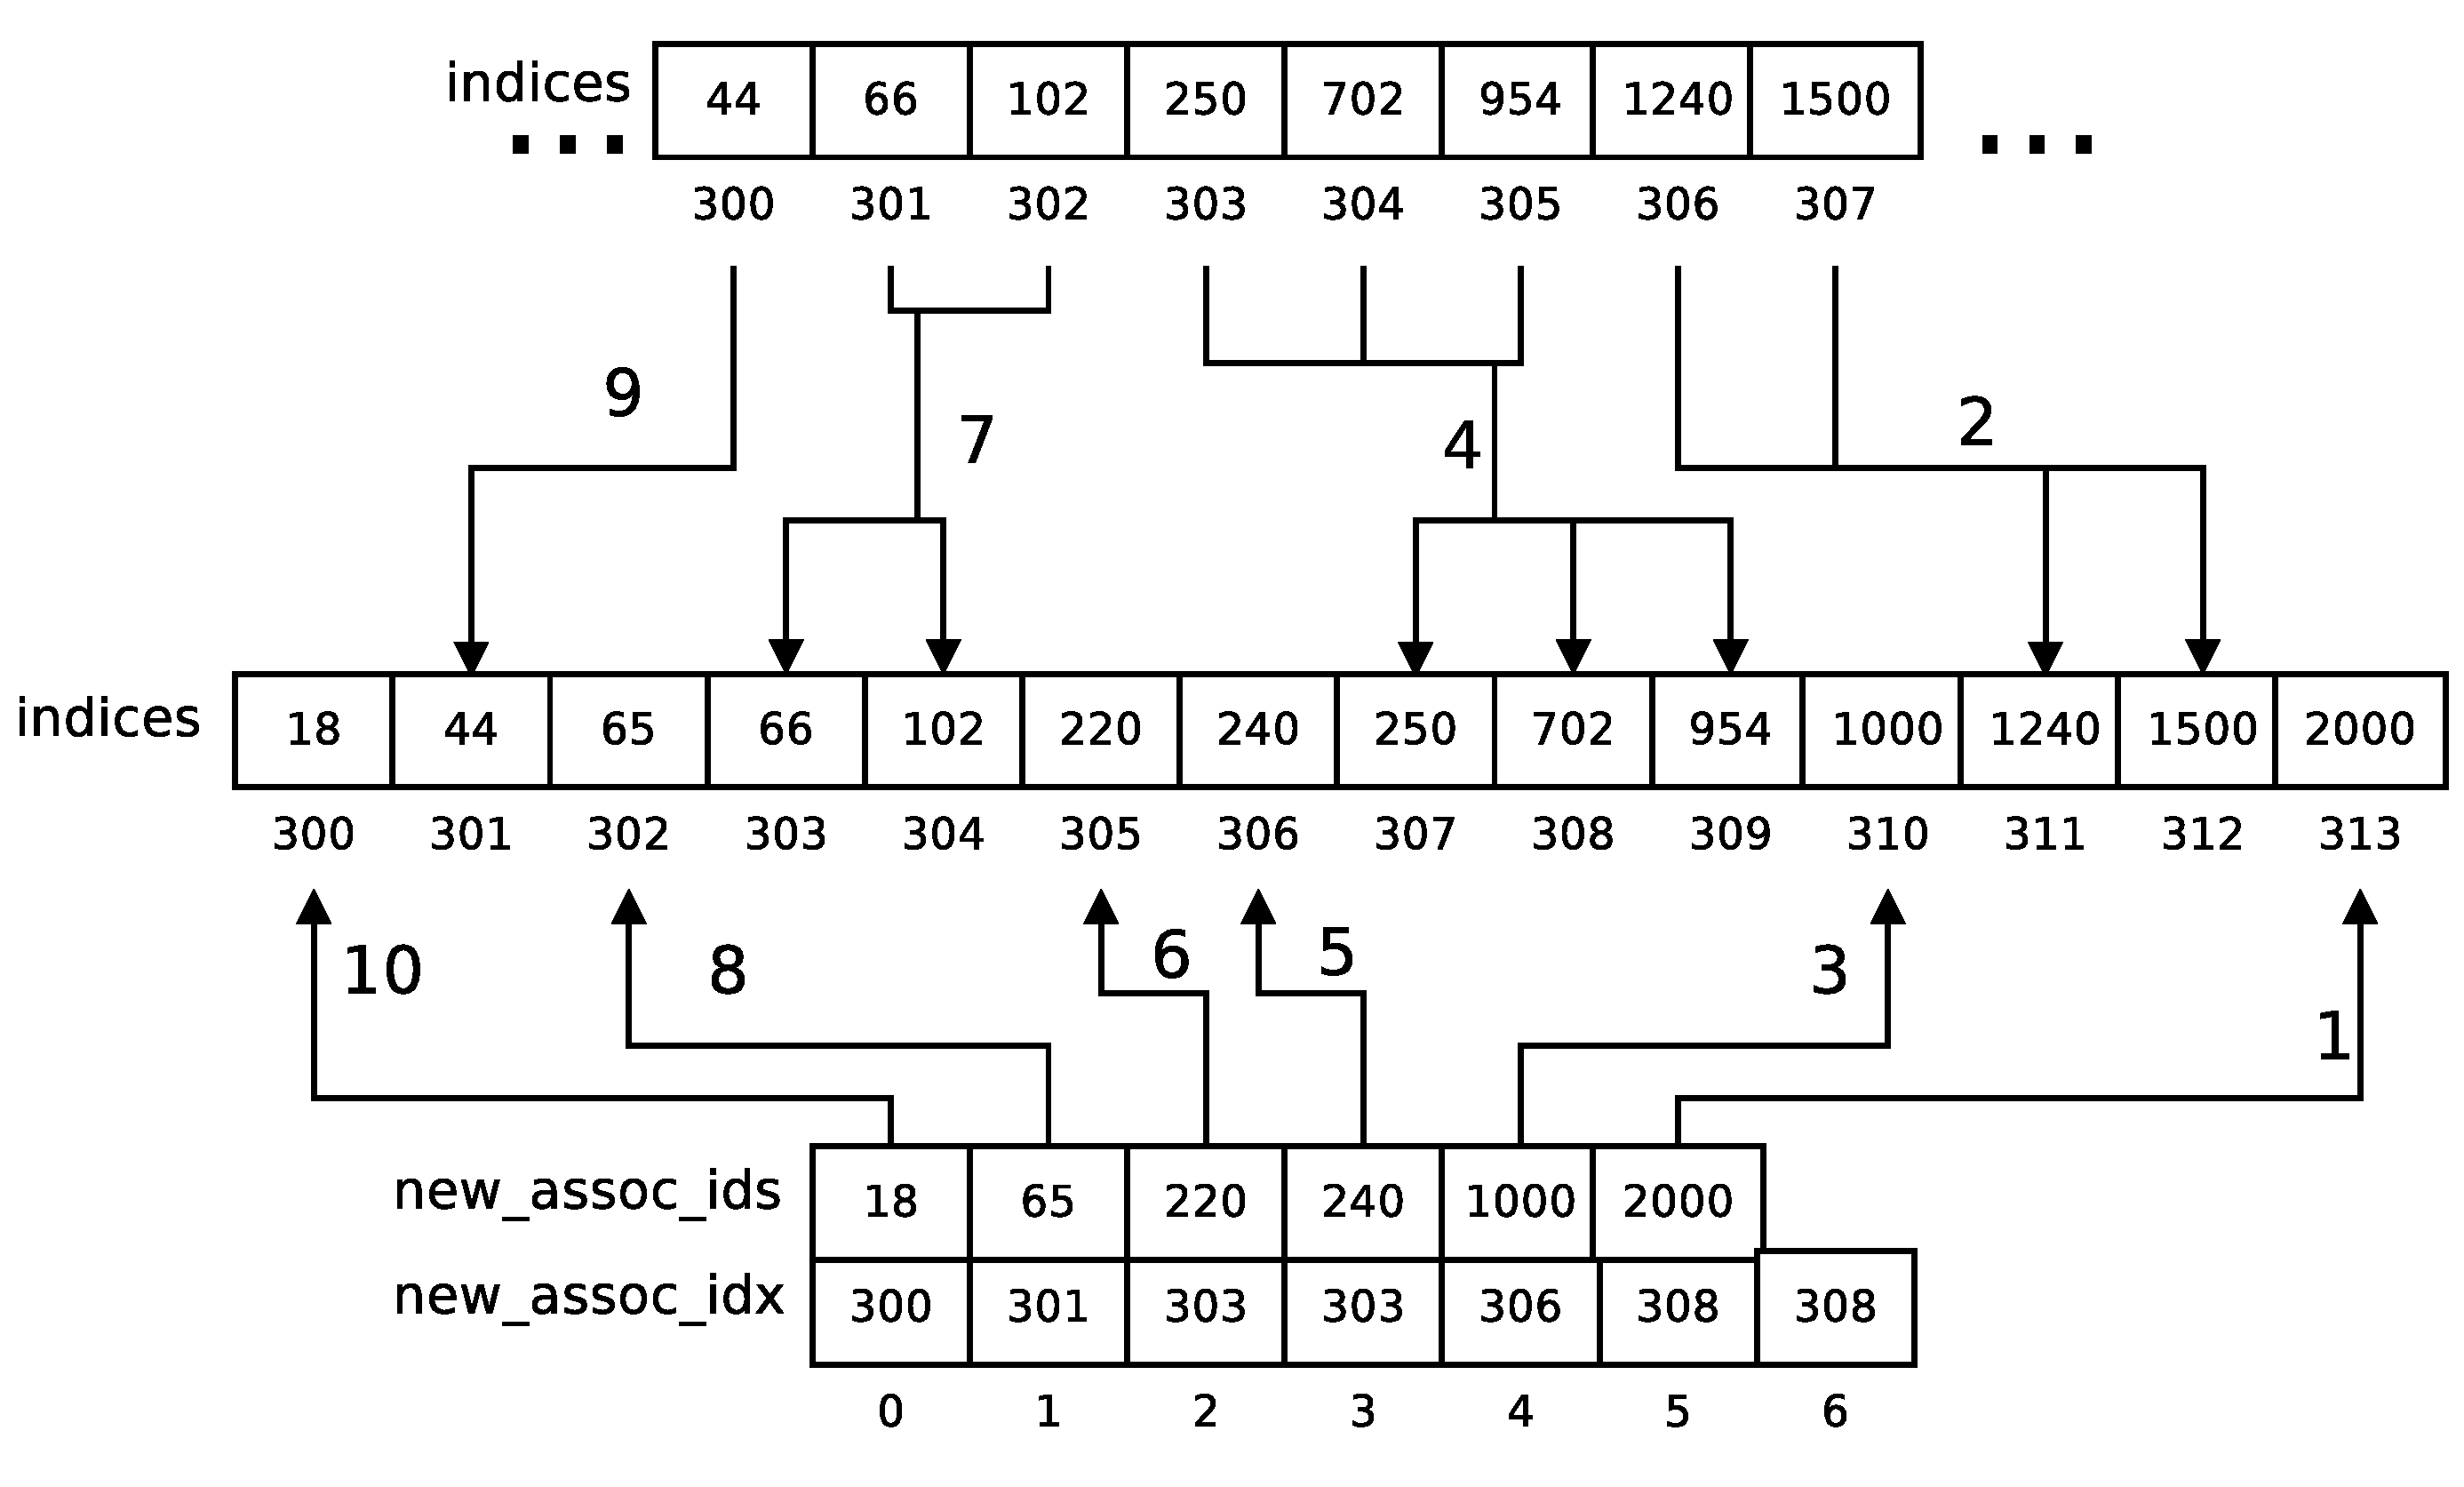
\includegraphics[width=0.45\textwidth]{methodology/sorted_insert}
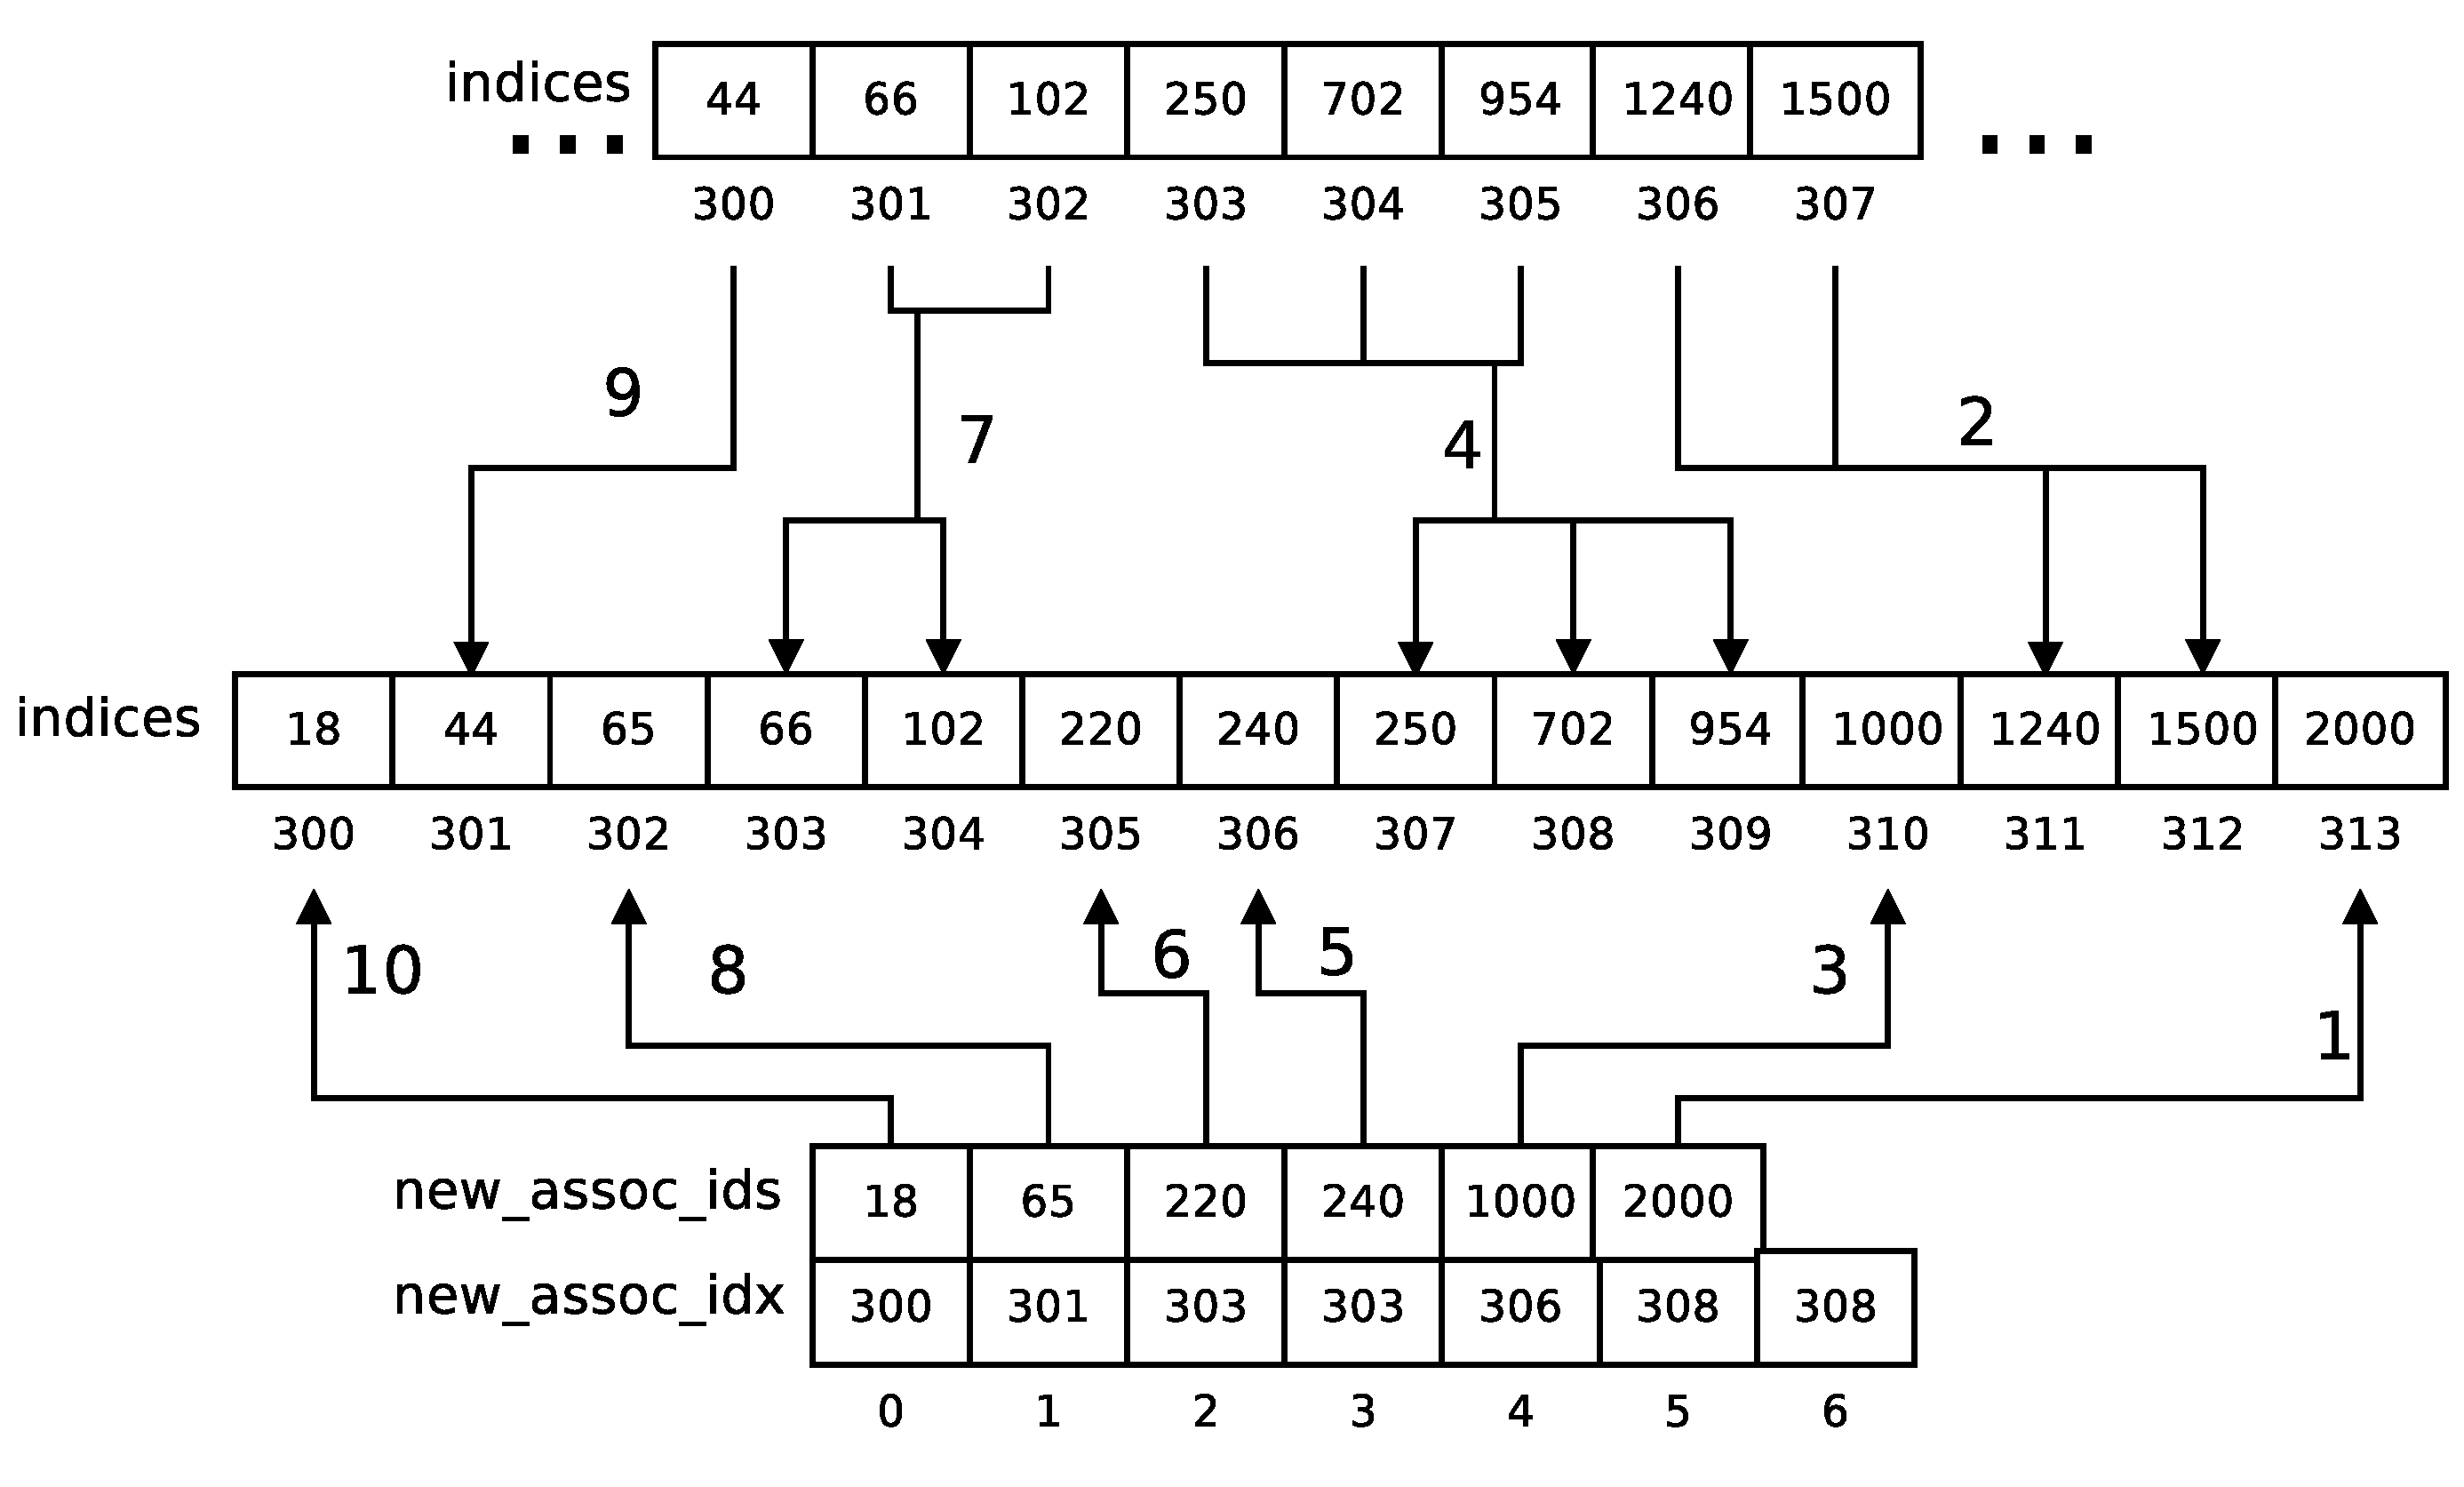
\includegraphics[width=\columnwidth]{methodology/sorted_insert}
\caption{Inserting a cluster from a partition in the co-association matrix. The arrows indicate to where the indices are moved. The numbers indicate the order of the operation.}
\label{fig:normal part}
\end{figure}


The new associations have to be added to the pattern's \emph{indices} interval in a sorted manner.
The number of associations corresponding to the $i$-th pattern (\emph{degree[i]}) is incremented by the amount of new associations to be added.
During the sorting process a pointer to the current index to add associations $o\_ptr$ is kept (it is initialized to the new total number of associations of a pattern).
The sorting mechanism looks at two consecutive elements in the \emph{new\_assoc\_idx} array, starting from the end.
If the $i$-th element of the \emph{new\_assoc\_idx} array is greater or equal than the $(i-1)$-th element, then all the associations in the \emph{indices} array between them (including the first element) are shifted to the right by $i$ positions. %are copied to the end of the \emph{indices} interval. %, i.e. they are shifted to the right by $i$ positions.
Then, or in case the comparison fails, the $(i-1)$-th element of the \emph{new\_assoc\_ids} is copied to the \emph{indices} array in the position specified by \emph{o\_ptr}.
The \emph{o\_ptr} pointer is decremented anytime an association is written in the \emph{indices} array.
This showed to be roughly twice as fast as using an implementation of \emph{quicksort}.

% After each pass on a cluster (adding or incrementing all associations to a pattern in the cluster), the new associations have to be added to the pattern's \emph{indices} interval in a sorted manner.
% The number of associations corresponding to the $i$-th pattern (\emph{degree[i]}) is incremented by the amount of new associations to be added.
% %The new interval of the \emph{indices} array belonging to the $i$-th pattern now has \emph{degree[i]} plus the number of new associations.
% An element is added to the end of the \emph{new\_assoc\_idx} array with the value of \emph{degree[i]} so that the last new association can be included in the general cycle.
% During the sorting process a pointer to the current index to add associations $o\_ptr$ is kept ( it is initialized to the new total number of associations of a pattern).
% The sorting mechanism looks at two consecutive elements in the \emph{new\_assoc\_idx} array, starting from the end.
% If the $i$-th element of the \emph{new\_assoc\_idx} array is greater or equal than the $(i-1)$-th element, then all the associations in the \emph{indices} array between them (including the first element) are copied to the end of the \emph{indices} interval, i.e. they are shifted to the right by $i$ positions.
% Then, or in case the comparison fails, the $(i-1)$-th element of the \emph{new\_assoc\_ids} is copied to the \emph{indices} array in the position specified by \emph{o\_ptr}.
% The \emph{o\_ptr} pointer is decremented anytime an association is written in the \emph{indices} array.
% This showed to be roughly twice as fast as using an implementation of \emph{quicksort}.

\subsection{EAC CSR Condensed}

A further reduction of space complexity in the EAC CSR scheme is possible by building only the upper triangular, since this completely describes the co-association matrix.
This means that the amount of associations decreases as one goes further down the matrix.
Instead of pre-allocating the same amount of associations for each pattern, the pre-allocation follows the same pattern of the number of associations, effectively reducing the space complexity.
The strategy used was a linear one, where the first $5\%$ of patterns have access to $100\%$ of the the estimated maximum number of associations, the last pattern has access to $5\%$ of that value and the number available for the patterns in between decreases linearly from $100\%$ to $5\%$.

%!TEX root = bare_jrnl.tex
%%%%%%%%%%%%%%%%%%%%%%%%%%%%%%%%%%%%%%%%%%%%%%%%%%%%%%%%%%%%%%%%%%%%%%
%     File: ExtendedAbstract_imple.tex                               %
%     Tex Master: ExtendedAbstract.tex                               %
%                                                                    %
%     Author: Andre Calado Marta                                     %
%     Last modified : 27 Dez 2011                                    %
%%%%%%%%%%%%%%%%%%%%%%%%%%%%%%%%%%%%%%%%%%%%%%%%%%%%%%%%%%%%%%%%%%%%%%
% A Calculation section represents a practical development
% from a theoretical basis.
%%%%%%%%%%%%%%%%%%%%%%%%%%%%%%%%%%%%%%%%%%%%%%%%%%%%%%%%%%%%%%%%%%%%%%

\section{Optimization of the recovery step of EAC}
\label{sec:recovery}


Two candidates were considered for the final step of EAC.
A SL based on a GPU version of MST \cite{Sousa2015} was implemented.
Although the GPU MST algorithm showed speed-up on benchmark datasets, the co-association matrix is typically less sparse than those, which made any speed-up impossible.
External algorithms were the second candidate solution.
This solution is based on storing the co-association matrix on disk, performing the expensive computation (memory and speed wise) of \emph{argsort} and then processing the matrix in batches until the final MST is extracted.

% The co-association matrix can become very large for large datasets.
% Even using the EAC CSR method to reduce memory usage, the memory used occupies a significant portion of main memory.

% The algorithm to compute a MST brings additional space complexity that make it infeasible to perform the final partition recovery on a large co-association matrix in main memory.
% External memory algorithms address this issue.
% % out of core processing %TODO check
% External memory algorithms refers to algorithms that are based on disk (or other large capacity but typically low latency storage technology), usually by loading small batches to main memory, processing them, saving the results and repeat until the whole computation is done.
% This section describes the process of building the MST with low memory usage.
% The details of converting the MST in a Single-Link clustering are described in chapter \ref{chapter:stateofart} and omitted here.

\subsection{Kruskal's algorithm and implementation}

% Kruskal algorithm
The MST algorithm used was Kruskal.
The original paper of Kruskal's \cite{kruskal1956shortest} algorithm describes three approaches for finding a MST.
The SciPy library offers an efficient implementation for the following construct (taken directly from the original paper of Kruskal's algorithm):
\begin{displayquote}
CONSTRUCTION A. Perform the following step as many times as possible: Among the edges of G not yet chosen, choose the shortest edge which does not form any loops with those edges already chosen. Clearly the set of edges eventually chosen must form a spanning tree of G, and in fact it forms a shortest spanning tree.
\end{displayquote}
If the graph $G$ if connected, the algorithm will stop before processing all edges when $|V| - 1$ edges are added to the MST, where $V$ is the set of edges.
This implementation works on a sparse matrix in the CSR format.

One of the main steps of the implementation is computing the order of the edges of the graph without sorting the edges themselves, an operation called \emph{argsort}.
To illustrate this, the \emph{argsort} operation on the array $ \left [  4 , 5 , 2 , 1, 3 \right ]$ would yield $ \left [  3 , 2 , 4, 0 , 1 \right ]$ since the the smallest element is at position 3 (starting from 0), the second smalled at position 2, etc.
% This operation is useful to avoid computing the edge with minimum (\emph{min}) weight in every iteration.
% Doing so would increase time complexity since a sorting algorithm may have an average time complexity to $O(n log n)$ (QuickSort algorithm) while a single minimum has a time complexity of $O(n)$.
% Computing the minimum at every iteration when every edge must be processed means that there will be $|E|$ iterations and so the total time complexity for the minimum operation alone will be $O(E ^ E)$ if processed edges are only given the maximum value possible or $O(E!)$ if they are removed.
% These time complexities are much higher than a $O(E log E)$.
% The result of this operation is an array of length $|E|$ (i.e. the number of associations in EAC), which means it will occupy at least the same size as the array containing the weights of the edges.
This operation is much less time intensive than computing the shortest edge at each iteration.
However, the total space used is typically 8 times larger for EAC since the data type of the weights uses only one byte and the number of associations is very large, forcing the use of a 8 byte integer for the \emph{argsort} output array.
This is the real motivation to store the co-association matrix in disk and use an external sorting algorithm.

\subsection{Kruskal's implementation with an external sorting algorithm}

The \emph{PyTables} library \cite{pytables}, which is built on top of the \emph{HDF5} format \cite{hdf5}, was used for storing the graph, performing the external sorting for the \emph{argsort} operation and loading the graph in batches for processing.
This implementation starts by storing the CSR graph to disk.
However, instead of saving the \emph{indptr} array directly, it stores an expanded version of the same length as the \emph{indices} array, where the $i$-th element contains the origin vertex (or row) of the $i$-th edge.
This way, a binary search for discovering the origin vertex becomes unnecessary.

Afterwards, the \emph{argsort} operation is performed by building a completely sorted index (CSI) \cite{AltetiAbad2007} of the \emph{data} array of the CSR matrix.
It should be noted that the arrays themselves are not sorted.
Instead, the CSI allows for a fast indexing of the arrays in a sorted manner (according to the order of the edges).
%The CSI will be used to retrieve edges from the stored graph in a sorted manner.
The process of building the CSI has a very low main memory usage and can be disregarded in comparison to the co-association matrix.

The SciPy implementation of Kruskal's algorithm was modified to work with batches of the graph.
This was easily implemented just by making the additional data structures used in the building of MST persistent between iterations.
The new implementation loads the graph in batches and in a sorted manner, e.g. first load a batch of the 1000 shortest edges, then a batch of the next 1000 shortest edges, etc.
Each batch must be processed sequentially since the edges must be processed in a sorted manner, which means there is no possibility for parallelism in this process.
Typically, the batch size is a very small fraction of the size of the edges, so the total memory usage for building the MST is overshadowed by the size of the co-association matrix.
The time complexity for building the CSI is higher that of computing the \emph{argsort} operation, but the formal time complexity is not reported in the source \cite{AltetiAbad2007}.
As an example, for a $500 \: 000$ vertex graph the SL-MST approach took $54.9$ seconds while the external memory approach took $2613.5$ seconds - 2 orders of magnitude higher.
\section{\uppercase{Results}}
\label{sec:resul}

Results presented here originated from one of three machines, that will be referred to as Alpha, Bravo and Charlie.
The main specifications of each machine are as follows:
\begin{itemize}
  \item \textbf{Alpha}: 4 GBs of main memory, a 2 core Intel i3-2310M 2.1GHz CPU and a NVIDIA GT520M with 1 GB;
  \item \textbf{Bravo}: 32 GBs of main memory, a 6 core Intel i7-4930K 3.4GHz CPU and a NVIDIA Quadro K600 with 1 GB;
  \item \textbf{Charlie}: 32 GBs of main memory, a 4 core Intel i7-4770K 3.5GHz CPU and a NVIDIA K40c with 12 GB.
\end{itemize}

%%%%%%%%%%%%%%%%%%%%%%%%%%%%%%%%%%%%%%%%%%%%%%%%%%%%%%%%%%%%%%%%%%%%%%
\subsection{GPU Parallel K-Means}

Both sequential and parallel versions of K-Means were executed over a wide spectrum of datasets varying number of patterns, features and centroids.
All tests were executed on machine Charlie and the block size was maintained constant at 512.
Whenever the number of clusters was superior to $70\%$ of the number of patterns (e.g. 800 clusters for a dataset with 1000 pattern), that particular test case was not executed.


Observing Figures \ref{fig:kmeans dim 2} and \ref{fig:kmeans dim 200}, it is clear that the number of patterns, features and clusters influence the speed-up.
For the simple case of 2 dimensions (Fig \ref{fig:kmeans dim 2}), the speed-up increases with the number of patterns.
However, there is no speed-up when the overall complexity of the datasets is low.
For 2 clusters, there is no speed-up before $100 \: 000$ patterns.
And even after that mark, the speed-up is not significant.
On the other hand, for a large number of clusters, there is speed-up for any number of patterns executed.
Not only that, that speed-up is highest for a superior number of clusters.
The reason for this is that the total amount of work increases linearly with the number of clusters but is diluted by the number of threads that can execute simultaneously.

\begin{figure}[hbtp]
    \centering
    \includegraphics[width=\columnwidth]{{{2_0}}}
    \caption{Speed-up of the labeling phase for datasets of 2 dimensions and varying the number of patterns and clusters. The dotted black line represents a speed-up of one.}
    \label{fig:kmeans dim 2}
\end{figure}

However, as the dimensionality increases (observe Fig. \ref{fig:kmeans dim 200}), the speed-up increases until a certain number of patterns and then decreases.
Here, the initial number of patterns for which there is a speed-up is lower and the number of clusters plays less an influence on the speed-up.
We believe the reason for this is related to the implementation itself.
The current parallel implementation does not use shared memory, which is fast.
As such, for every computation, each thread fetches the relevant data from global memory which is significantly slower.
As the number of dimensions increases, the amount of data that each thread must fetch also increases.
Furthermore, since the number of dimensions affects both data points and centroids, if the number of dimensions increases by 2 the number of fetches to memory increases by 4.
So, the speed-up increases with the dataset complexity until a point where the number of fetches to memory starts having a very significant effect on the execution time and it decreases close to $50\%$.

\begin{figure}[hbtp]
    \centering
    \includegraphics[width=\columnwidth]{{{200_0}}}
    \caption{Speed-up of the labeling phase for datasets of 200 dimensions and varying the number of patterns and clusters. The dotted black line represents a speed-up of one.}
    \label{fig:kmeans dim 200}
\end{figure}

%%%%%%%%%%%%%%%%%%%%%%%%%%%%%%%%%%%%%%%%%%%%%%%%%%%%%%%%%%%%%%%%%%%%%%
\subsection{Validation with original implementation}

The results of the original version of EAC, implemented in Matlab, are compared with those of the proposed solution.
Several small datasets, chosen from the datasets used in \cite{Lourenco2010} and taken from the UCI Machine Learning repository \cite{Lichman:2013}, were processed by the two versions of EAC.
Furthermore, since the generation of the ensemble is probabilistic and can change the results between runs, the proposed version is processed with the ensembles created by the original version as well.
This guarantees that the combination and recovery phases of EAC, which are deterministic when using SL, are equivalent to the original.
All data in this section refers to processing done in machine Alpha.
Table \ref{tab:validation error acc} presents the difference between the accuracies of the two versions.
Analyzing these results, it is apparent that the difference is minimal, most likely due the original version using Matlab and the proposed using Python.
Moreover, a speed-up as low as 6 and as high as 200 was obtained over the original version in the various steps, including the production step. %, even for these small datasets.

% It should be noted at this point that the original implementation always maps the dissimilarities of the co-association matrix to the range $\left [ 0 , 1 \right ]$.
% This forces the co-association matrix to have a floating point data type.
% However, since the number of partitions used is usually less than 255, the proposed version uses unsigned integers of 1 byte to reduce the used memory considerably.
% The differences in accuracy are thought to come from rounding differences of the two frameworks used and from this difference in data type.

\begin{table}[h]
\centering
\caption{Difference between accuracy of the two implementations of EAC, using the same ensemble. Accuracy was measured using the H-index \cite{Meila2003}.}

\begin{tabular}{lll}
\toprule
         &        \multicolumn{2}{c}{Number of clusters scheme} \\
Dataset &      Fixed & Lifetime \\
\midrule
breast\_cancer &  4.948755e-06 &     2.825769e-06 \\
ionosphere     &  1.652422e-06 &     1.452991e-06 \\
iris           &  3.333333e-06 &     3.333333e-06 \\
isolet         &  1.038861e-07 &     4.084904e-07 \\
optdigits      &  3.795449e-06 &     1.480513e-06 \\
pima           &  3.333333e-06 &     3.333333e-06 \\
pima\_norm     &  4.166667e-07 &     4.166667e-07 \\
wine\_norm     &  1.123596e-07 &     1.910112e-06 \\
\bottomrule
\end{tabular}

\label{tab:validation error acc}
\end{table}

%%%%%%%%%%%%%%%%%%%%%%%%%%%%%%%%%%%%%%%%%%%%%%%%%%%%%%%%%%%%%%%%%%%%%%
\subsection{Set-up for large dataset testing}
% It was suggested before that $K_{min}$ would influence other properties of EAC.
% This includes the execution times of the production, combination and recovery phases.
The results here presented refer to a synthetic large dataset comprised by a mixture of 6 Gaussians, where 2 pairs are overlapped and 1 pair is touching.
This dataset was sampled into several smaller datasets to cover a wider range of number of patterns.

Different rules for computing the $K_{min}$, different co-association matrix formats and different approaches for the final clustering will be mentioned.
The different rules and their aliases are presented in Table \ref{tab:eac rules}.
The different formats for the co-association matrix are the \emph{full} (for fully allocated $n \times n$ matrix), \emph{full condensed} (for a fully allocated $\frac{n(n-1)}{2}$ array to build the upper triangular matrix), \emph{sparse complete} (for EAC CSR), \emph{sparse condensed const} (for EAC CSR building only the upper triangular matrix) and \emph{sparse condensed linear} (for EAC CSR condensed).
The different approaches for the final clustering are \emph{SLINK} \cite{Sibson1973}, \emph{SL-MST} (for using the Kruskal implementation in SciPy) and \emph{SL-MST-Disk} for the modified version that performs an external memory sort.

\begin{table}[h]
\centering
\caption{Different rules for computing $K_{min}$ and $K_{max}$. $n$ is the number of patterns and $sk$ is the number of patterns per cluster.}

\begin{tabular}{lcc}
\toprule
Rule &  $K_{min}$ &  $K_{max}$ \\
\midrule
\emph{sqrt}     & $\frac{\sqrt{n}}{2}$      & $\sqrt{n}$    \\
\emph{2sqrt}    & $\sqrt{n}$                & $2 \sqrt{n}$  \\
\emph{sk=sqrt2} & $sk = \frac{\sqrt{n}}{2}$ & $1.3 K_{min}$ \\
\emph{sk=300}   & $sk = 300$                & $1.3 K_{min}$ \\
\bottomrule
\end{tabular}

\label{tab:eac rules}
\end{table}


The experiment that generated the results of these section was set up as follows.
A large dataset was generated.
The dataset was sampled uniformly to produce a smaller dataset with the desired number of patterns.
A clustering ensemble was produced (production phase) for each of these smaller datasets and for each of the rules, using K-Means.
From each ensemble, co-association matrices of every applicable format were built (combination phase).
A matrix format was not applicable when the dataset complexity would make its correspondent co-association matrix too big to fit in main memory.
The final clustering (recovery phase) was also done for each of the matrix formats.
The number of clusters was chosen with the lifetime criteria \cite{Fred2005}.
SL-MST was not executed if its space complexity was too big to fit in main memory.
Furthermore, the combination and recovery phases were repeated several times for smaller datasets for statistical relevant of the execution times, so as to make the influence of any background process less salient.
For big datasets, the execution times are big enough that the influence of background processes is negligible.
All results presented here originated from machine Bravo.
The same analysis that is presented here was performed on a similar dataset with separated Gaussians, from which similar conclusions were drawn.

\subsection{Execution times}

Execution times are related with the $K_{min}$ parameter, whose evolution is presented in Fig. \ref{fig:eac kmin evo}.
Rules \emph{sqrt}, \emph{2sqrt} and \emph{sk=sqrt2} never intersect but rule $sk=300$ intersects all of them, finishing with the highest $K_{min}$.
Observing Fig. \ref{fig:eac ensemble times}, one can see that the same thing happens to the production execution time associated with the $sk=300$ rule and the inverse happens to the combination time (Fig. \ref{fig:eac build rules}).
A higher $K_{min}$ means more centroids for each K-Means run to compute, so it is not surprising that the execution time for computing the ensemble increases as $K_{min}$ increases.

\begin{figure}[hbt!]
    \centering
    \includegraphics[width=0.8\columnwidth]{{{kmin_evolution}}}
    \caption{Evolution of $K_{min}$ with the number of patterns for different rules.}
    \label{fig:eac kmin evo}
\end{figure}

\begin{figure}[hbt!]
    \centering
    \includegraphics[width=0.8\columnwidth]{{{ensemble_time}}}
    \caption{Execution time for the production of the clustering ensemble.}
    \label{fig:eac ensemble times}
\end{figure}

\begin{figure}[hbt!]
    \centering
    \includegraphics[width=0.8\columnwidth]{{{build_sparse_condensed_linear}}}
    \caption{Execution time for building the co-association matrix from ensemble with different rules.}
    \label{fig:eac build rules}
\end{figure}

Fig. \ref{fig:eac build matrices} shows the execution times on a longitudinal study for optimized matrix formats.
It is clear that the sparse formats are significantly slower than the fully allocated ones, specially for smaller datasets.
The \emph{full condensed} format usually takes close to half the time than the \emph{full} format, which is natural given that it performs half the operations.
Idem for the \emph{sparse condensed} formats compared to the \emph{sparse complete}.
The big discrepancy between the sparse and full formats is due to the fact that the former needs to do a binary search at each association update and needs to keep the internal sparse data structure sorted.

\begin{figure}[hbt!]
    \centering
    \includegraphics[width=0.8\columnwidth]{{{2sqrt}}}
    \caption{Execution time for building the co-association matrix with different matrix formats.}
    \label{fig:eac build matrices}
\end{figure}

%\subsection{Performance comparison between SLINK, SL-MST and SL-MST-Disk}

The clustering times of the different methods of SL discussed previously (SLINK, SL-MST and SL-MST-Disk) are presented in Figures \ref{fig:eac sl} and \ref{fig:eac sl-mst}.
The SL-MST-Disk method is significantly slower than any of the other methods.
This is expected, since it uses the hard drive which has very slow access times compared to main memory.
SL-MST is faster than SLINK, since it processes zero associations while SL-MST takes advantage of a graph representation and only processes the non-zero associations.
In resemblance to what happened with combination times, the condensed variants take roughly half the time has their complete counterparts, since SL-MST and SL-MST-Disk over condensed co-association matrices only process half the number of associations.
Although this is not depicted, SLINK takes roughly the same time for every rule, which means $K_{min}$ has no influence.
% This comes as no surprise, since SLINK processes both zero and non-zero associations and $K_{min}$ only influences the number of non-zero associations.
This comes as no surprise, since SLINK processes the whole matrix, regardless of its association sparsity.
The same rationale can be applied to SL-MST, where different rules can have significant influence over execution time, since they change the total number of associations.
As with the combination phase, the execution time referent to the \emph{sk=300} rule started with the greatest time and decreased with an increase in the number of patterns until it was the fastest.

\begin{figure}[hbt!]
    \centering
    \includegraphics[width=0.8\columnwidth]{{{slink_vs_sl-mst}}}
    \caption{Comparison between the execution times of the three methods of SL. SLINK runs over fully allocated condensed matrix while SL-MST and SL-MST-Disk run over the condensed and complete sparse matrices.}
    \label{fig:eac sl}
\end{figure}

\begin{figure}[hbt!]
    \centering
    \includegraphics[width=0.8\columnwidth]{{{sl_mem_time_sparse_condensed_linear}}}
    \caption{Comparison between the execution times of SL-MST for different rules.}
    \label{fig:eac sl-mst}
\end{figure}

The execution times of all phases combined are presented in Figures \ref{fig:eac total mem} and \ref{fig:eac total disk}.
The results are presented for the \emph{sparse condensed linear} format but the remaining results follow the same pattern.
It is interesting to note that, when using the SL-MST method in the recovery phase, the execution time for three of the rules do not differ much.
This is due to a sort of balancing between a slowing down of the production phase and a speeding up of the combination and recovery phases as the $K_{min}$ increases at a higher rate for $sk=300$ than for other rules.
This is not observed for the $sqrt$ rule as $K_{min}$ is always low enough that the total time is always dominated by the combination and recovery phases.
The same does not happen when using the SL-MST-Disk method, as the total time is completely dominated by the recovery phase.
This is clear, since the results in Fig. \ref{fig:eac total disk} follow a pattern similar to that presented in Fig. \ref{fig:eac sl-mst}.


\begin{figure}[hbt!]
    \centering
    \includegraphics[width=0.8\columnwidth]{{{total_time_sl-mst}}}
    \caption{Execution times for all phases combined, using SL-MST in the recovery phase.}
    \label{fig:eac total mem}
\end{figure}

\begin{figure}[hbt!]
    \centering
    \includegraphics[width=0.8\columnwidth]{{{total_time_sl-mst-disk}}}
    \caption{Execution times for all phases combined, using SL-MST-Disk in the recovery phase.}
    \label{fig:eac total disk}
\end{figure}


\subsection{Analysis of the number of associations}

The sparse nature of EAC has been referred to before and is clearer in Fig. \ref{fig:eac assoc density}.
This figure shows the association density, i.e. number of associations relative to the $n^2$ associations in a full matrix.
The \emph{full condensed} format has a constant density of $49.5\%$.
Idem for the \emph{sparse complete} and \emph{sparse condensed} formats, as long as no associations are discarded.
The overall tendency is for the density to decrease as the number of patterns of the dataset increases, since the \emph{full} matrix grows quadratically.
Besides, it would be expected that the same associations would be grouped together more frequently in partitions and simply make previous connections stronger instead of creating new ones, if the relationship between the number of patterns and $K_{min}$ is constant.

% The sparse nature of EAC has been referred to before and is clearer in Fig. \ref{fig:eac assoc density}.
% This figure shows the association density, i.e. number of associations relative to the $n^2$ associations in a full matrix.
% The \emph{full condensed} format as a constant density of $49.5\%$ and the density of \emph{sparse complete} is two times that of the \emph{sparse condensed} formats.
% The overall tendency is for the density to decrease as the number of patterns of the dataset increases.
% This is to be expected since the \emph{full} matrix grows quadratically.
% Besides, it would be expected that the same associations would be grouped together more frequently in partitions and simply make previous connections stronger instead of creating new ones.
% Results presented in Fig. \ref{fig:eac assocs per pattern}, which presents the number of associations per pattern, suggest otherwise.
% The number of associations per pattern increases with the number of patterns of the dataset, with the notable exception of the \emph{sk=300} rule which increases until it reaches a certain limit and then stabilizes.
% This is explained by the fact that this rule is based on setting a maximum constant number ($300$) of patterns in any given cluster, while in the other rules this number increases with the number of patterns.
% The number of associations per pattern is not $300$ for the $sk=300$ rule because a pattern will be clustered with different neighbors in different partitions.
% Still, the number of neighbors doesn't change enough that the number of associations per pattern increases boundlessly.
% In fact, Fig. \ref{fig:eac assocs per pattern} suggests that the number of associations per pattern is around 3 times the upper bound on the number of patterns per cluster (strictly related to $K_{min}$).
% This is clearer for $sk=300$, but if one would trace the the number of patterns divided by $K_{min}$ for each rule, the contribution is close.
% \cite{Lourenco2010} reported that, on average, \"the overall contribution of the clustering ensemble (including unbalanced clusters) duplicates the co-associations produced in a single balanced clustering with Kmin clusters\".
% The spectrum of datasets evaluated regarding the number of patterns was smaller than that evaluated in the present work.
% The present results suggest a slightly higher value.
% So, the decrease in density is more related with the quadratic growth of the \emph{full} matrix in contrast with a linear growth of the number of associations.

\begin{figure}[hbt!]
    \centering
    \includegraphics[width=0.8\columnwidth]{{{assoc_density_sparse_condensed_linear}}}
    \caption{Density of associations relative to the full co-association matrix, which hold $n^2$ associations.}
    \label{fig:eac assoc density}
\end{figure}

% \begin{figure}[hbt!]
%     \centering
%     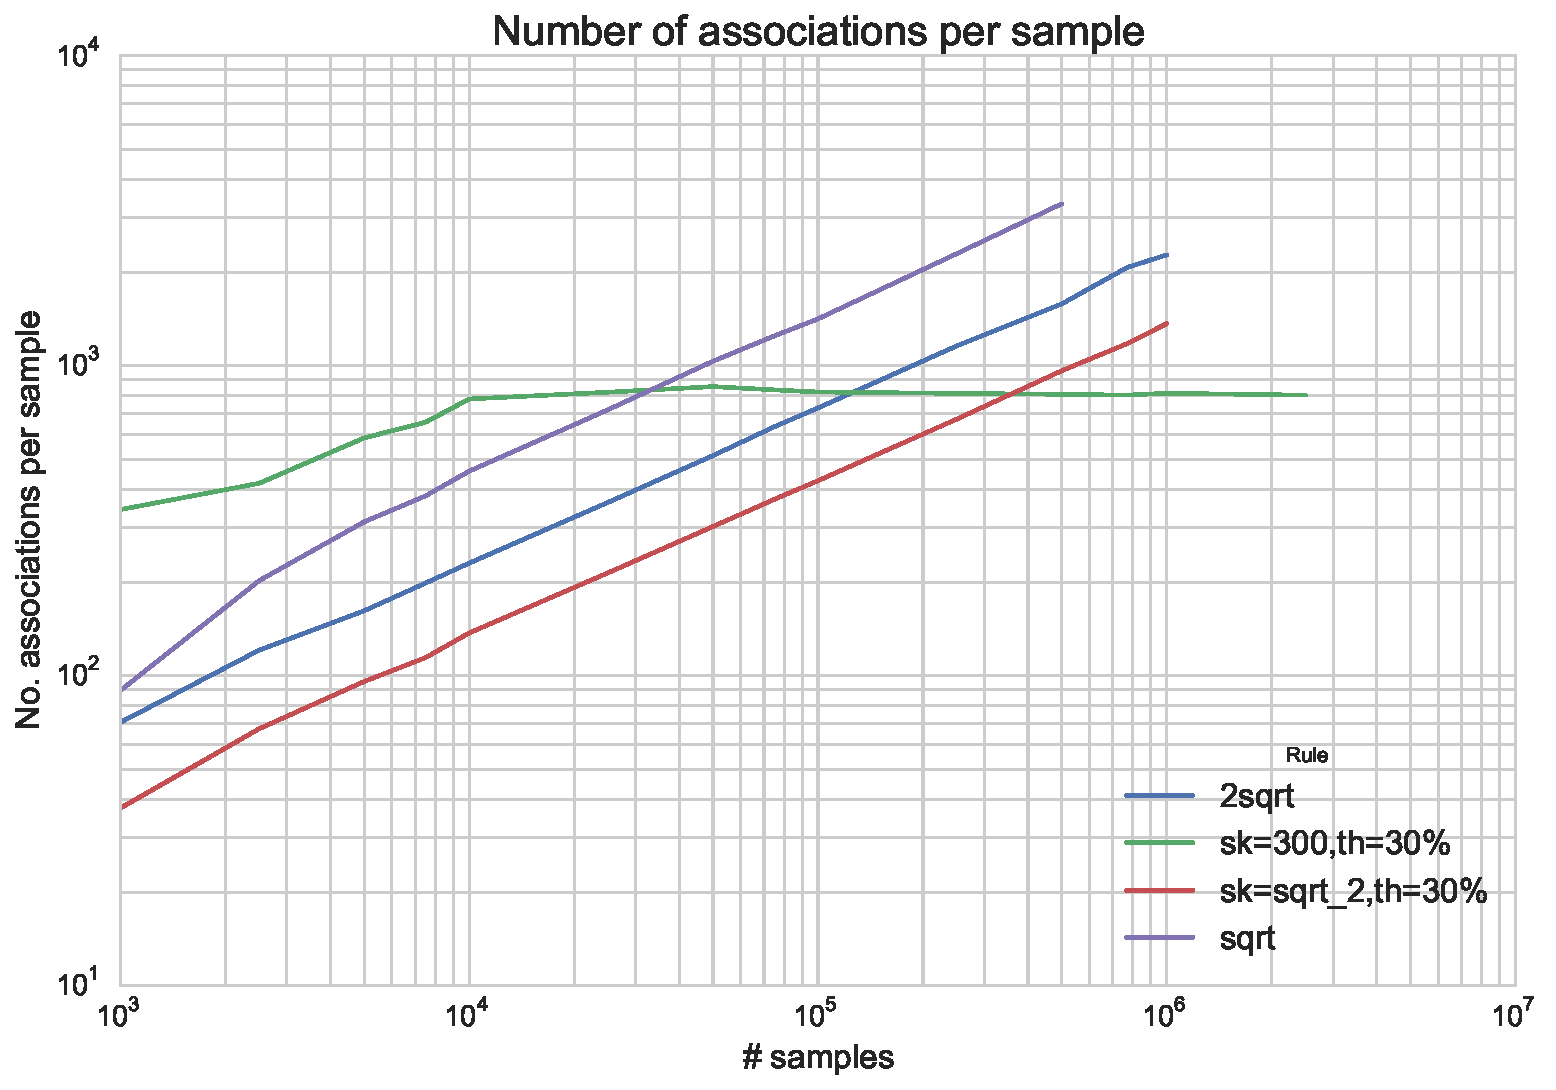
\includegraphics[width=0.8\columnwidth]{{{results/eac/assocs_per_sample}}}
%     \caption{Evolution of the total number of associations divided by the number of patterns according to the different rules.}
%     \label{fig:eac assocs per pattern}
% \end{figure}

Predicting the number of associations before building the co-association matrix is useful for coming up with combination schemes that are both memory and speed efficient.
It was stated before that the biggest cluster size in any partition of the ensemble is a good parameter for this end.
Fig. \ref{fig:eac max assocs bgs} presents the relationship between the biggest cluster size and the maximum number of associations of any pattern.
These ratio increases with the number of patterns in the beginning, but as the number of patterns increases it never goes over 3.

\begin{figure}[hbt!]
    \centering
    \includegraphics[width=0.8\columnwidth]{{{max_assoc_bgs}}}
    \caption{Maximum number of associations of any pattern divided by the number of patterns in the biggest cluster of the ensemble.}
    \label{fig:eac max assocs bgs}
\end{figure}

However, the number of features of the used datasets is rather reduced.
It might be the case that this ratio would increase with the number of features, since there would be more degrees where the clusters might include other neighbors.
With this in mind, further studies ranging a wider spectrum of datasets should yield more enlightening conclusions or reinforce those presented here.

\subsection{Space complexity}

As explained previously, the allocated space for the space formats is based on a prediction that uses the biggest cluster size of the ensemble.
This allocated space is usually more than what is necessary to store the total number of associations, to keep a safety margin.
Furthermore, the CSR sparse format, on which the EAC CSR strategy is based, requires an array of the same size of the predicted number of associations.
This overhead may in fact make the sparse format pre-allocate more associations than are actually possible for some rules and in very small datasets.
Still, the allocated number of associations becomes a very small fraction compared to the \emph{full} matrix as the dataset complexity increases, which is the typical case for using a sparse format.
The actual memory used is presented in Fig. \ref{fig:eac mem density}.
Here, the data types used play a big role in the amount of memory that is required.
The associations can be stored in a single byte, since the number of partitions is usually less than 255.
This means that the memory used by the fully allocated formats is $n^2$ and $\frac{n(n-1)}{2}$ Bytes for the complete and condensed versions, respectively.
In the sparse formats, the values of the associations are also stored in an array of unsigned integers of 1 Byte.
However, an array of integers of 4 bytes of the same size must also be kept to keep track of the destination pattern each association belongs to.
Besides, one other array of integers of 8 bytes is kept but it is negligible compared to the other two arrays.
The impact of the data types can be seen for smaller datasets where the total memory used is actually significantly higher than that of the \emph{full} matrix.
It should be noted that this discrepancy is not as high for other rules as for $sk=300$.
Still, the sparse formats, and in particular the condensed sparse format, is preferred since the memory used for large datasets is a small fraction of what would be necessary if using any of the fully allocated formats.

\begin{figure}[hbt!]
    \centering
    \includegraphics[width=0.8\columnwidth]{{{sk_300}}}
    \caption{Memory used relative to the full $n^2$ matrix. The \emph{sparse complete} and \emph{sparse condensed const} curves are overlapped.}
    \label{fig:eac mem density}
\end{figure}
\section{\uppercase{Conclusions}}
\label{sec:conc}
\noindent The main goal of scaling the EAC method for larger datasets than was previously possible was achieved.
The EAC method is composed by three steps and, to scale the whole method, each step was optimized separately.
In the process, EAC was also optimized for smaller datasets.
In essence, the main contributions to the EAC method, by step, were the GPU parallel K-Means, the EAC CSR strategy and the SL-MST-Disk.
%In essence, the main contributions to the EAC method, by step, were the GPU parallel K-Means in the production step, the EAC CSR strategy in the combination step and the SL-MST-Disk in the recovery step.
New rules for $K_{min}$ were tested and the effects that these rules have on other properties of EAC were studied.
Together, these contributions allow for the application of EAC to datasets whose complexity was not handled by the original implementation.

Further work involves thorough evaluation in real world problems.
Additional work may include further optimization of the Parallel GPU K-means by using shared memory and a better sorting of the co-association graph in \emph{SL-MST-Disk}.
%By using using bigger chunks in main memory and possibly even using the GPU, sorting the co-association graph should become significantly faster.

\section*{\uppercase{Acknowledgments}}
\noindent This work was supported by the Portuguese Foundation for Science and Technology, scholarship number SFRH/BPD/103127/2014, and grant PTDC/EEI-SII/7092/2014.



%\vfill
\bibliographystyle{apalike}
{\small
\bibliography{library}}

\vfill
\end{document}